\documentclass[11pt,aspectratio=169]{beamer}

\usepackage{booktabs}
\usepackage{array}
\usepackage{tikz}
\usepackage{pgfplots}
\usepgfplotslibrary{fillbetween}
\usepackage{xcolor}
\usepackage{amsmath}
\usepackage{mathtools}
\usepackage{siunitx}
\usetikzlibrary{positioning,calc,arrows.meta,decorations.pathreplacing}
\pgfplotsset{compat=1.18}

\usetheme[titleformat=smallcaps,progressbar=frametitle]{metropolis}
\definecolor{UTburnt}{HTML}{BF5700}
\definecolor{LBJnavy}{HTML}{172A46}
\definecolor{softgray}{HTML}{F2F3F5}
\definecolor{midgray}{HTML}{6B7280}
\definecolor{softorange}{HTML}{F9E7DA}
\setbeamercolor{alerted text}{fg=UTburnt}
\setbeamercolor{frametitle}{bg=LBJnavy,fg=white}
\setbeamercolor{progress bar}{fg=UTburnt,bg=gray!25}
\setbeamercolor{block title}{bg=LBJnavy!10,fg=LBJnavy}
\setbeamercolor{block body}{bg=softgray}
\setbeamertemplate{navigation symbols}{}
\setbeamertemplate{itemize item}{\color{UTburnt}$\blacktriangleright$}
\setbeamertemplate{itemize subitem}{\color{UTburnt}$\bullet$}

\author{Sergio I. Garc\'ia-R\'ios}
\title{Normal and Binomial Distributions}
\subtitle{Models for continuous outcomes and repeated yes/no trials}
\institute{PA 311N: Data Analysis for Public Policy\\LBJ School of Public Affairs}
\date{September 28, 2026}

\newcommand{\yourturn}[1]{%
\begin{center}
\begin{minipage}{0.90\textwidth}
\begin{alertblock}{Your Turn}
#1
\end{alertblock}
\end{minipage}
\end{center}}

\newcommand{\ourturn}[1]{%
\begin{center}
\begin{minipage}{0.90\textwidth}
\begin{block}{Our Turn}
#1
\end{block}
\end{minipage}
\end{center}}

\begin{document}

% 1
\begin{frame}[plain]
\centering
\vspace{0.7cm}
{\color{LBJnavy}\LARGE\bfseries Normal and Binomial Distributions\par}
\vspace{0.45cm}
{\large Models for continuous outcomes and repeated yes/no trials\par}
\vspace{1.0cm}
{\normalsize Sergio I. Garc\'ia-R\'ios\par}
\vspace{0.2cm}
{\small PA 311N: Data Analysis for Public Policy\par}
{\small LBJ School of Public Affairs\par}
\vfill
{\small September 28, 2026\par}
\end{frame}

% 2
\begin{frame}{From single events to distributions}
Last time we asked questions like:
\[
P(A), \qquad P(A\mid B), \qquad P(A\cap B).
\]

Today we ask a different kind of question:

\begin{center}
\Large What values can a \alert{random variable} take,\\and how likely is each value?
\end{center}

\vfill
A probability distribution gives us a model for the full range of possible outcomes.
\end{frame}

% 3
\begin{frame}{Today: two models for uncertainty}
\begin{enumerate}
  \item \textbf{Probability distributions} organize possible values and their probabilities.
  \item The \textbf{normal distribution} models many continuous, symmetric outcomes.
  \item \textbf{Z-scores} put observations on a common standard-deviation scale.
  \item The \textbf{binomial distribution} models counts of successes in repeated binary trials.
\end{enumerate}

\vfill
We will move back and forth between \alert{pictures}, \alert{formulas}, and \alert{R}.
\end{frame}

% 4
\begin{frame}{A random variable turns outcomes into numbers}
A \alert{random variable} assigns a numerical value to the outcome of a random process.

\vspace{0.6em}
Suppose we randomly select 4 households eligible for a weatherization program.

\begin{itemize}
  \item Each household either completes enrollment or does not.
  \item Let $X$ = number of households that complete enrollment.
\end{itemize}

Then
\[
X\in\{0,1,2,3,4\}.
\]

\vfill
The uncertainty is no longer just ``success or failure.'' It is about the \alert{value of $X$}.
\end{frame}

% 5
\begin{frame}{A probability distribution describes the random variable}
A probability distribution tells us:

\begin{enumerate}
  \item which values the random variable can take; and
  \item the probability attached to those values or ranges of values.
\end{enumerate}

\vspace{0.8em}
Every probability distribution must obey:
\[
0\leq P(\text{event})\leq 1
\]
and the probabilities across all possible outcomes must total 1.

\vfill
Different kinds of random variables require different kinds of distributions.
\end{frame}

% 6
\begin{frame}{Discrete and continuous distributions}
\begin{columns}[T,onlytextwidth]
\column{0.47\textwidth}
\textbf{Discrete}
\begin{itemize}
  \item Separate, countable values
  \item We can assign probability to an exact value
  \item Example: number of households enrolled
  \item Binomial distribution
\end{itemize}

\column{0.47\textwidth}
\textbf{Continuous}
\begin{itemize}
  \item Values along a continuum
  \item Probability comes from intervals, not exact points
  \item Example: height or a test score model
  \item Normal distribution
\end{itemize}
\end{columns}

\vfill
\alert{Discrete: probability at values. Continuous: probability over ranges.}
\end{frame}

% 7
\begin{frame}{Your turn: discrete or continuous?}
\yourturn{Classify each random variable.
\begin{enumerate}
  \item Number of 311 calls received in one hour
  \item Time required to process a permit application
  \item Number of surveyed residents who support a proposal
  \item Household annual income
\end{enumerate}}

\pause
\vfill
\begin{center}
\small Discrete, continuous, discrete, continuous.
\end{center}
\end{frame}

% 8
\begin{frame}{The normal distribution is a family of curves}
A normal distribution is characterized by two parameters:
\[
X\sim N(\mu,\sigma)
\]

\begin{itemize}
  \item $\mu$ determines the \alert{center}.
  \item $\sigma$ determines the \alert{spread}.
  \item The curve is symmetric and unimodal.
  \item Total area under the curve equals 1.
\end{itemize}

\vfill
Changing $\mu$ moves the curve. Changing $\sigma$ stretches or compresses it.
\end{frame}

% 9
\begin{frame}{The 68--95--99.7 rule}
\begin{center}
\begin{tikzpicture}
\begin{axis}[
  width=0.88\textwidth,height=0.50\textheight,
  axis lines=middle,
  xmin=-3.6,xmax=3.6,ymin=0,ymax=0.44,
  xtick={-3,-2,-1,0,1,2,3},
  xticklabels={$\mu-3\sigma$,$\mu-2\sigma$,$\mu-\sigma$,$\mu$,$\mu+\sigma$,$\mu+2\sigma$,$\mu+3\sigma$},
  ytick=\empty,
  xlabel={},ylabel={},
  tick label style={font=\scriptsize}
]
\addplot[name path=normal,domain=-3.5:3.5,samples=200,very thick,LBJnavy]{1/sqrt(2*pi)*exp(-x^2/2)};
\path[name path=axis] (axis cs:-3.5,0) -- (axis cs:3.5,0);
\addplot[UTburnt!25] fill between[of=normal and axis,soft clip={domain=-1:1}];
\end{axis}
\end{tikzpicture}
\end{center}

\vspace{-0.4em}
\begin{center}
\begin{tabular}{ccl}
Within $1\sigma$ & $\approx 68\%$ & of observations \\
Within $2\sigma$ & $\approx 95\%$ & of observations \\
Within $3\sigma$ & $\approx 99.7\%$ & of observations
\end{tabular}
\end{center}
\end{frame}

% 10
\begin{frame}{Your turn: use the empirical rule}
Suppose scores on a large assessment are approximately normal with
\[
\mu=70,\qquad \sigma=10.
\]

\yourturn{
Without a calculator, approximately what proportion of scores fall:
\begin{enumerate}
  \item between 60 and 80?
  \item between 50 and 90?
  \item above 80?
\end{enumerate}}

\pause
\vfill
\[
\boxed{68\%},\qquad \boxed{95\%},\qquad \boxed{16\%}.
\]
\end{frame}

% 11
\begin{frame}{Z-scores put observations on a common scale}
A z-score tells us how many standard deviations an observation falls above or below the mean:
\[
\boxed{z=\frac{x-\mu}{\sigma}}
\]

\begin{itemize}
  \item $z=0$: exactly at the mean
  \item $z=1$: one standard deviation above the mean
  \item $z=-2$: two standard deviations below the mean
\end{itemize}

\vfill
Z-scores remove the original units and replace them with \alert{standard-deviation units}.
\end{frame}

% 12
\begin{frame}{Our turn: standardize an observation}
Suppose assessment scores have
\[
\mu=70,\qquad \sigma=10.
\]
A student scores 88.

\[
z=\frac{88-70}{10}=\boxed{1.8}
\]

\ourturn{Interpret $z=1.8$ in words.}

\pause
The score is \alert{1.8 standard deviations above the mean}.
\end{frame}

% 13
\begin{frame}{Z-scores let us compare different scales}
Consider two observations:

\begin{columns}[T,onlytextwidth]
\column{0.46\textwidth}
\textbf{Assessment A}
\[
\mu=70,\;\sigma=10,\;x=90
\]
\[
z=2
\]

\column{0.46\textwidth}
\textbf{Assessment B}
\[
\mu=500,\;\sigma=50,\;x=600
\]
\[
z=2
\]
\end{columns}

\vfill
The raw scores are not comparable, but both observations occupy the same relative position in their distributions.
\end{frame}

% 14
\begin{frame}{Important distinction: z-scores vs. normal probabilities}
You can calculate a z-score for \alert{any} quantitative distribution with a mean and standard deviation.

\vspace{0.7em}
But translating a z-score into a normal probability requires an approximately normal model.

\begin{alertblock}{Do not skip the shape}
A z-score of 2 always means ``two SDs above the mean.'' It does \textbf{not} always mean that only about 2.5\% of observations are above it.
\end{alertblock}

\vfill
This is why we looked at distributions before calculating summaries earlier in the course.
\end{frame}

% 15
\begin{frame}{For a continuous distribution, probability is area}
\begin{center}
\begin{tikzpicture}
\begin{axis}[
  width=0.82\textwidth,height=0.50\textheight,
  axis lines=middle,
  xmin=-3.5,xmax=3.5,ymin=0,ymax=0.44,
  xtick={-2,-1,0,1,2},
  xticklabels={$-2$,$-1$,$0$,$1$,$2$},
  ytick=\empty,
  tick label style={font=\small}
]
\addplot[name path=normal2,domain=-3.5:3.5,samples=200,very thick,LBJnavy]{1/sqrt(2*pi)*exp(-x^2/2)};
\path[name path=axis2] (axis cs:-3.5,0) -- (axis cs:3.5,0);
\addplot[UTburnt!40] fill between[of=normal2 and axis2,soft clip={domain=1:3.5}];
\end{axis}
\end{tikzpicture}
\end{center}

\[
P(Z>1)\approx 0.159.
\]

The probability is the \alert{area under the curve} over the region we care about.
\end{frame}

% 16
\begin{frame}{R automates normal probabilities}
For $X\sim N(70,10)$, what is the probability that $X>80$?

\begin{block}{R}
\ttfamily
1 - pnorm(80, mean = 70, sd = 10)
\end{block}

\[
P(X>80)\approx \boxed{0.1587}.
\]

\vfill
\begin{itemize}
  \item \texttt{pnorm()} gives area to the \alert{left}.
  \item For an upper tail, use $1-$ that area.
\end{itemize}
\end{frame}

% 17
\begin{frame}{Normal is a model, not a default}
Some variables are approximately symmetric and bell-shaped. Others are not.

\begin{columns}[T,onlytextwidth]
\column{0.47\textwidth}
\textbf{Normal model may be reasonable}
\begin{itemize}
  \item adult height in a homogeneous population
  \item some standardized measurement errors
  \item some large-scale assessment scores
\end{itemize}

\column{0.47\textwidth}
\textbf{Often not normal}
\begin{itemize}
  \item household income
  \item emergency-room wait time
  \item counts of events
  \item heavily bounded or skewed outcomes
\end{itemize}
\end{columns}

\vfill
\alert{Look at the variable before choosing the model.}
\end{frame}

% 18
\begin{frame}[standout]
\Large Repeated yes/no trials lead to a different model.
\end{frame}

% 19
\begin{frame}{The binomial random variable counts successes}
Suppose a city outreach program has a 60\% enrollment-completion rate among eligible households.

We randomly select 4 households and define
\[
X=\text{number that complete enrollment}.
\]

Possible values are
\[
X\in\{0,1,2,3,4\}.
\]

\vfill
The individual outcome is binary. The \alert{binomial random variable} counts how many successes occur across repeated trials.
\end{frame}

% 20
\begin{frame}{When can we use a binomial model? Think BINS}
A binomial model requires:

\begin{description}
  \item[\textbf{B}] \textbf{Binary} outcome on each trial: success/failure.
  \item[\textbf{I}] \textbf{Independent} trials.
  \item[\textbf{N}] Fixed \textbf{number} of trials, $n$.
  \item[\textbf{S}] \textbf{Same} probability of success, $p$, on each trial.
\end{description}

\vfill
If these conditions hold, then
\[
X\sim \operatorname{Binom}(n,p).
\]
\end{frame}

% 21
\begin{frame}{Your turn: is a binomial model appropriate?}
\yourturn{A city randomly samples 20 permit applications and counts how many are approved within 10 business days. Can we model the count as binomial? What would you need to assume?}

\pause
\vfill
We need a binary outcome, fixed $n=20$, approximately independent applications, and a common probability $p$ of timely approval.

\vspace{0.5em}
The formula is easy. The model assumptions require judgment.
\end{frame}

% 22
\begin{frame}{Exactly two successes in four trials}
Suppose $p=0.60$ and $n=4$. What is
\[
P(X=2)?
\]

One possible sequence is
\[
S,S,F,F.
\]

Its probability is
\[
(0.60)^2(0.40)^2=0.0576.
\]

\vfill
But there are several different sequences with exactly two successes.
\end{frame}

% 23
\begin{frame}{How many sequences produce exactly $k$ successes?}
With $n=4$ and $k=2$, the possible success positions are:
\[
SSFF,\; SFSF,\; SFFS,\; FSSF,\; FSFS,\; FFSS.
\]

There are 6 sequences.

In general, the number of ways to choose $k$ success positions from $n$ trials is
\[
\boxed{{n\choose k}=\frac{n!}{k!(n-k)!}}.
\]

\vfill
For $n=4,k=2$:
\[
{4\choose 2}=6.
\]
\end{frame}

% 24
\begin{frame}{The binomial probability formula}
For $X\sim\operatorname{Binom}(n,p)$,
\[
\boxed{P(X=k)={n\choose k}p^k(1-p)^{n-k}}
\]

Think of the formula as two pieces:

\begin{enumerate}
  \item \alert{Probability of one particular sequence}: $p^k(1-p)^{n-k}$
  \item \alert{Number of sequences}: ${n\choose k}$
\end{enumerate}

\vfill
\[
P(X=k)=\text{number of ways}\times\text{probability of each way}.
\]
\end{frame}

% 25
\begin{frame}{Our turn: exactly two of four}
For $n=4$, $p=0.60$, and $k=2$:
\begin{align*}
P(X=2)
&={4\choose 2}(0.60)^2(0.40)^2\\
&=6(0.36)(0.16)\\
&=\boxed{0.3456}.
\end{align*}

\ourturn{Interpret 0.3456 in words.}

\pause
About 34.6\% of repeated groups of four would contain exactly two completions under this model.
\end{frame}

% 26
\begin{frame}{Your turn: exactly four of five}
Suppose $X\sim\operatorname{Binom}(5,0.60)$.

\yourturn{Calculate $P(X=4)$ by hand. Identify $n$, $k$, $p$, and $1-p$ before substituting.}

\pause
\begin{align*}
P(X=4)
&={5\choose4}(0.60)^4(0.40)^1\\
&=5(0.1296)(0.40)\\
&=\boxed{0.2592}.
\end{align*}
\end{frame}

% 27
\begin{frame}{R automates exact binomial probabilities}
The R function is \texttt{dbinom()}:

\begin{block}{R}
\ttfamily
dbinom(4, size = 5, prob = 0.60)
\end{block}

\[
P(X=4)=0.2592.
\]

\vfill
The arguments map directly onto the model:
\begin{itemize}
  \item first argument: $k$, desired number of successes
  \item \texttt{size}: $n$, number of trials
  \item \texttt{prob}: $p$, probability of success
\end{itemize}
\end{frame}

% 28
\begin{frame}{Exactly, at most, and at least are different questions}
For $X\sim\operatorname{Binom}(20,0.60)$:

\begin{align*}
P(X=15) &\quad \text{exactly 15}\\
P(X\leq 15) &\quad \text{at most 15}\\
P(X\geq 15) &\quad \text{at least 15}
\end{align*}

\vfill
\begin{block}{R}
\ttfamily
\begin{tabular}{ll}
dbinom(15, 20, .60) & \# exactly 15\\
pbinom(15, 20, .60) & \# at most 15\\
1 - pbinom(14, 20, .60) & \# at least 15
\end{tabular}
\end{block}
\end{frame}

% 29
\begin{frame}{A binomial distribution has a center and spread}
If
\[
X\sim\operatorname{Binom}(n,p),
\]
then
\[
\boxed{\mu=np}
\]
and
\[
\boxed{\sigma=\sqrt{np(1-p)}}.
\]

\vfill
These formulas describe the distribution of the \alert{count of successes} across repeated samples.
\end{frame}

% 30
\begin{frame}{Our turn: expected completions in 20 households}
Suppose
\[
X\sim\operatorname{Binom}(20,0.60).
\]

Expected number of completions:
\[
\mu=np=20(0.60)=\boxed{12}.
\]

Standard deviation:
\[
\sigma=\sqrt{20(0.60)(0.40)}\approx\boxed{2.19}.
\]

\vfill
This does \textbf{not} mean every group of 20 contains exactly 12 successes. It describes the center and typical variation across repeated groups.
\end{frame}

% 31
\begin{frame}{What does the binomial distribution look like?}
\begin{center}
\begin{tikzpicture}
\begin{axis}[
  width=0.88\textwidth,height=0.52\textheight,
  ybar,bar width=7pt,
  xmin=4.5,xmax=20.5,ymin=0,ymax=0.20,
  xtick={5,6,...,20},
  ytick={0,.05,.10,.15,.20},
  ylabel={$P(X=k)$},xlabel={Number of successes, $k$},
  tick label style={font=\scriptsize},
  axis line style={midgray},
  ymajorgrids=true,grid style={gray!15}
]
\addplot[fill=UTburnt!70,draw=UTburnt] coordinates {
(5,0.0012945) (6,0.0048544) (7,0.0145631) (8,0.0354974)
(9,0.0709949) (10,0.1171416) (11,0.1597385) (12,0.1797058)
(13,0.1658823) (14,0.1244117) (15,0.0746470) (16,0.0349908)
(17,0.0123497) (18,0.0030874) (19,0.0004875) (20,0.0000366)
};
\draw[dashed,very thick,LBJnavy] (axis cs:12,0) -- (axis cs:12,0.19);
\end{axis}
\end{tikzpicture}
\end{center}

\vspace{-0.3em}
For $n=20,p=.60$, the distribution is centered at $np=12$.
\end{frame}

% 32
\begin{frame}{Why normal and binomial appear in the same lecture}
As $n$ grows, many binomial distributions become increasingly smooth and bell-shaped.

A common rule of thumb checks the expected number of successes and failures:
\[
np\geq10
\qquad\text{and}\qquad
n(1-p)\geq10.
\]

For $n=20,p=.60$:
\[
np=12,\qquad n(1-p)=8.
\]

\vfill
So this example is \alert{not quite} in the comfortable range for a normal approximation.
\end{frame}

% 33
\begin{frame}{Two distributions, two kinds of questions}
\begin{center}
\renewcommand{\arraystretch}{1.35}
\begin{tabular}{p{0.23\textwidth}p{0.31\textwidth}p{0.31\textwidth}}
\toprule
 & \textbf{Normal} & \textbf{Binomial} \\
\midrule
Variable & continuous & count of successes \\
Parameters & $\mu,\sigma$ & $n,p$ \\
Probability & area over intervals & probability at integer counts \\
R functions & \texttt{pnorm()} & \texttt{dbinom()}, \texttt{pbinom()} \\
Key check & shape is plausible & BINS conditions hold \\
\bottomrule
\end{tabular}
\end{center}
\end{frame}

% 34
\begin{frame}{Exit check}
\yourturn{
For each statement, identify the model or calculation you would use.
\begin{enumerate}
  \item A score is 1.5 standard deviations above its mean.
  \item Exactly 7 of 10 independent respondents support a proposal, with $p=.60$.
  \item A variable is strongly right-skewed. Should you automatically use a normal model?
  \item In a binomial model with $n=50,p=.30$, what is the expected number of successes?
\end{enumerate}}

\pause
\vfill
\begin{center}
Z-score; binomial; no; $np=15$.
\end{center}
\end{frame}

% 35
\begin{frame}{What I want you to leave with}
\begin{enumerate}
  \item A \textbf{distribution} describes the possible values of a random variable and how probability is allocated across them.
  \item The \textbf{normal model} is continuous, symmetric, and summarized by $\mu$ and $\sigma$.
  \item A \textbf{z-score} measures distance from the mean in standard-deviation units.
  \item The \textbf{binomial model} counts successes when BINS conditions hold.
  \item The formulas matter, but choosing the right model comes first.
\end{enumerate}

\vfill
\begin{center}
\Large \alert{Identify the variable. Check the model. Calculate. Interpret.}
\end{center}
\end{frame}

\end{document}
